\documentclass[11pt]{amsart}
\usepackage[all]{xy}
\usepackage[dvips]{graphicx}
\usepackage{amsfonts}
\usepackage{amssymb,latexsym,amsmath}
\usepackage{amsthm}
\usepackage{color}
\usepackage{empheq}
\usepackage{float}
\usepackage{hyperref}
\usepackage{listings}
\usepackage{mathrsfs}
\usepackage{slashed}
\usepackage{tikz}

\definecolor{dkgreen}{rgb}{0,0.6,0}
\definecolor{gray}{rgb}{0.5,0.5,0.5}
\definecolor{mauve}{rgb}{0.58,0,0.82}

\theoremstyle{definition}
\newtheorem{remark}{Remark}

\lstset{frame=tb,
    language=python,
    aboveskip=3mm,
    belowskip=3mm,
    showstringspaces=false,
    columns=flexible,
    basicstyle={\small\ttfamily},
    numbers=left,
    numberstyle=\tiny\color{gray},
    keywordstyle=\color{blue},
    commentstyle=\color{dkgreen},
    stringstyle=\color{mauve},
    breaklines=true,
    breakatwhitespace=true,
    tabsize=3
}

\textwidth = 420pt
\oddsidemargin = 18pt
\evensidemargin = 18pt

\begin{document}
\title{Cohort Revenue \& Retention Analysis: A Bayesian Approach}

\author{Juan Camilo Orduz}
\email{juanitorduz@gmail.com}
\urladdr{\href{https://juanitorduz.github.io/}{https://juanitorduz.github.io/}}
\address{Berlin, Germany}

\author{Daniel Guhl}
\email{daniel.guhl@hu-berlin.de}
\address{Humboldt-Universit\"{a}t zu Berlin, Germany}

\date{\today}

\begin{abstract}
    We present a Bayesian framework for jointly modeling cohort-level retention and revenue over time. We contribute a
    framework that couples these two business metrics through the number of active users. We model retention non-parametrically using
    Bayesian additive regression trees (BART) and Bayesian neural networks to capture non-linear patterns and seasonality, and couple
    this with a gamma-distributed revenue model where the estimated active user counts from the retention component inform
    the revenue predictions. This approach enables information sharing across cohorts, naturally incorporates seasonal effects,
    and provides well-calibrated uncertainty quantification through highest density intervals. The framework is flexible enough
    to incorporate additional covariates (which can vary over time) in both model components. We demonstrate the approach using synthetic
    data designed to reflect realistic business scenarios, showing accurate out-of-sample predictions with appropriate
    uncertainty estimates. The framework's modular design facilitates extensions to hierarchical structures: we demonstrate
    a multi-market implementation that pools information across markets with varying data availability, enabling reliable
    forecasts even for markets with very limited cohort histories. Implementation code is provided in PyMC and NumPyro, where
    we use both MCMC and stochastic variational inference to fit the models, making the method accessible for practical applications.
\end{abstract}

\maketitle

\tableofcontents

\addtocontents{toc}{\protect\setcounter{tocdepth}{1}}

\section{Introduction}
Understanding and predicting customer behavior directly impacts business profitability through improved retention strategies
and resource allocation. Among the metrics that define business success, retention and customer lifetime value
estimation stand at the forefront, serving as critical indicators of a company's ability to not only attract but maintain a
loyal customer base. These metrics transcend mere financial accounting—they represent the foundation upon which long-term
business strategies are built and refined. Seminal work by Fader and Hardie has established frameworks for both contractual
settings \cite{FaderHardie2007}, where subscription-based relationships predominate, and non-contractual settings
\cite{FaderHardie2005}, where customers may come and go without formal notification\footnote{Our definition of retention
    corresponds to what they call survival curve. See precise definitions below.}. Modern implementations of these CLV
models can now be found in Bayesian probabilistic programming frameworks such as PyMC (\cite{pymc2023}). Specifically, the
PyMC-Marketing library \cite{pymc_marketing} provides implementations of many standard buy-till-you-die (BTYD) models including
the BG/NBD, Pareto/NBD, and Gamma-Gamma models in a flexible, Bayesian framework. While these approaches have proven very valuable, they
often struggle to scale effectively. They can definitively be scaled with modern hardware and algorithms (for example,
stochastic variational inference, as described below). Nevertheless, this requires non-trivial work and effort.\\

For many decision-making processes, companies and senior management (think of a C-level executive) mostly need to understand
behaviors at the cohort level—groups (e.g. cohorts of customers who joined during the same time period). In this paper we
focus on this level of granularity. When shifting from individual to cohort-level analysis, businesses typically face a
methodological trilemma:

\begin{enumerate}
    \item \textbf{Complete pooling}: Aggregate all cohorts together and model retention and revenue as a collective whole,
          potentially obscuring important cohort-specific patterns.

    \item \textbf{No pooling}: Analyze each cohort in isolation, potentially overlooking valuable cross-cohort information
          and suffering from data sparsity for newer cohorts.

    \item \textbf{Partial pooling}: Model cohorts jointly with shared parameters, striking a balance between cohort-specific
          insights and statistical power.
\end{enumerate}

As detailed by \cite{FaderHardieNote2017}, each approach offers distinct advantages and limitations. However, a fundamental
challenge persists across these traditional methodologies: they typically lack the flexibility to efficiently incorporate
seasonality patterns and external regressors\footnote{Although, one can add regressors in some cases as described in
    \cite{FaderHardieNote2007} for the non-contractual case.}. This limitation becomes particularly problematic for businesses
with highly seasonal customer behavior—from retail operations affected by holiday shopping patterns to subscription services
influenced by annual promotional cycles. While some might argue that seasonality is secondary when estimating customer
lifetime value, the reality for many business models is that seasonal fluctuations significantly impact customer acquisition,
engagement, and retention decisions. Beyond the methodological challenges, businesses face practical hurdles in translating
retention and revenue models into actionable insights. Static models that fail to adapt to changing market dynamics or
consumer preferences quickly become outdated. Moreover, point estimates without associated uncertainty measures can lead to
misplaced confidence in business forecasts, potentially resulting in suboptimal resource allocation and strategic planning.
The Bayesian cohort-revenue-retention framework presented in this paper addresses these challenges and has been successfully
applied to real-world business datasets (both contractual and non-contractual settings). As we will describe below, the
model structure is flexible enough to incorporate extensive business specific prior knowledge through priors and convenient
parametrizations. Most importantly, the framework provides a straightforward way to add custom covariates in both the retention
and revenue components (and even in the coupling mechanism) which can vary over time. This is a fundamental advantage of this work,
as in other classical probabilistic models like BG/NBD and Pareto/NBD, covariates can be added but are computationally expensive
(and actually, the time-varying covariates require a significant amount of work to implement in a way that scales).


\subsection*{Why Cohort-Level Modeling?}

Before proceeding further, let's come back to the beginning and address an important question: why focus on cohort-level
rather than individual-level modeling? While individual-level models can provide granular predictions for specific customers,
cohort-level analysis offers several strategic advantages that make it particularly well-suited for many business
decision-making contexts.

\begin{itemize}

    \item First, cohort-level aggregation substantially reduces noise inherent in individual transaction data. Individual purchase
          patterns are often highly variable and influenced by idiosyncratic factors that average out when aggregating to the cohort
          level. This noise reduction leads to more stable parameter estimates and more reliable forecasts, particularly valuable for
          strategic planning where robustness is paramount.

    \item Second, cohort-level models align naturally with how many business decisions are actually made. Marketing strategies, budget
          allocations, and resource planning typically target customer segments rather than individuals. Financial forecasting and
          business planning operate at aggregate levels. A model that directly addresses these cohort-level questions provides more
          immediately actionable insights than individual-level predictions that must subsequently be aggregated. This alignment
          enhances accessibility for marketing stakeholders and strategic decision-makers who may not require customer-specific
          granularity but need to understand temporal patterns and cohort dynamics. For example, the model presented in this paper
          sucessfully enabeled data-driven decisions at a company operating in multiple countries where user-level predictions
          were hard to understand and make actionable. It was strategically better to segment the cohorts (adding other dimensions
          like marketing aquisition channel) to extract relevant signals and insights for senior management.

    \item Third, from a computational and practical perspective, cohort-level models scale more favorably than individual-level
          approaches, particularly as customer bases grow into millions. While modern Bayesian methods can handle large individual-level
          datasets, the computational requirements and implementation complexity increase substantially. Cohort-level modeling offers
          an efficient path to actionable insights without sacrificing the flexibility to incorporate rich covariate information when
          needed.

\end{itemize}

Importantly, the cohort-level focus does not preclude the incorporation of customer characteristics. As we demonstrate in our
framework, additional covariates—such as acquisition channel, geographic location, or customer segment—can be seamlessly
integrated into our model. To capture complex patterns in retention behavior without requiring explicit specification of
functional forms, we employ Bayesian Additive Regression Trees (BART) \cite{chipman2010bart}. BART is a flexible non-parametric
method that represents the unknown function as a sum of regression trees, allowing it to automatically learn non-linear
relationships and interactions between features. This flexibility is particularly valuable for cohort retention modeling, where
relationships between temporal features (cohort age, calendar time, seasonality) may be complex and difficult to specify
a priori. The non-parametric nature of BART allows it to scale effectively with many features, enabling the model to capture
heterogeneous effects across different customer types while maintaining the interpretability advantages of cohort-level
aggregation through tools like partial dependence plots. Thus, our approach strikes a balance: operating at the cohort level
for strategic clarity while retaining the flexibility to incorporate individual-level characteristics when they provide
additional explanatory power. Moreover, as we can additional imporse a hierarchical structure across markets or subset
of covariates, we can efficiently pool information across different cohorts and markets. Trying to do this pooling at
the individual level is essentially impossible to a scale of millions of customers (which is more the norm than the exception).

\subsection*{Visualizing Cohort Data}

To motivate the modeling approach, we first illustrate the type of data structures our framework is designed to handle.
Figure \ref{fig:retention_matrix} shows a typical cohort-level retention matrix. These cohorts are typically defined by 
business rules, e.g., customers who registered, downloaded the app, or made their first purchase during the same month.
Older cohorts have more historical data, and we would like to leverage this information to improve estimation for younger 
cohorts. That is, we do not want to model each cohort independently but rather the {\em whole retention matrix}.

\begin{figure}
    \centering
    \includegraphics[width=\textwidth]{images/revenue_retention_17_0.png}
    \caption{Retention matrix example. The matrix visualizes customer retention rates across different cohorts (rows) and
        observation periods (columns). Each cell represents the proportion of customers from a specific acquisition
        cohort that remained active in a subsequent period. Colors indicate retention rates, with darker colors typically
        showing higher retention. This visualization allows for identifying cohort-specific patterns, seasonal effects,
        and retention decay over time. The diagonal is excluded as it always contains trivial values of 1 (100\%
        retention) for the cohort's first period.}
    \label{fig:retention_matrix}
\end{figure}

Similarly, we want to model the corresponding revenue matrix (Figure \ref{fig:revenue_matrix}), ensuring we use all 
available information to improve revenue estimation for younger cohorts. A key observation is the strong correlation 
between revenue and the number of active users (Figure \ref{fig:active_users}), which motivates our coupling mechanism.

\begin{figure}
    \centering
    \includegraphics[width=\textwidth]{images/revenue_retention_23_0.png}
    \caption{Revenue per cohort. This heatmap visualizes the total revenue generated by each cohort (rows) across different
        time periods (columns). The color intensity corresponds to revenue magnitude, revealing a strong correlation
        with the number of active users (Figure \ref{fig:active_users}).}
    \label{fig:revenue_matrix}
\end{figure}

\begin{figure}
    \centering
    \includegraphics[width=\textwidth]{images/revenue_retention_21_0.png}
    \caption{Number of active users across cohorts. This heatmap displays the absolute count of active users for each
        cohort (rows) across observation periods (columns).}
    \label{fig:active_users}
\end{figure}

The rest of this paper is organized as follows. Section \ref{sec:related_work} reviews related work in age-period-cohort 
modeling, survival analysis, and customer lifetime value. Section \ref{sec:model_framework} presents our core theoretical 
contribution: a coupled retention-revenue framework where the number of active users links both components. 
Section \ref{sec:synthetic_example} instantiates the framework using synthetic data, including model diagnostics and 
in-sample/out-of-sample predictive performance evaluation.
Section \ref{sec:alternative_approaches} discusses alternative non-parametric approaches using neural networks. 
Section \ref{sec:hierarchical} extends the framework to hierarchical multi-market settings. Section \ref{sec:hm_application} 
validates the approach on real-world H\&M transaction data, followed by a discussion of model limitations and trade-offs in Subsection \ref{sec:limitations}. Finally, Section \ref{sec:conclusion} concludes.

%%%%%%%%%%%%%%%%%%%%%%%%%%%%%%%%%%%%%%%%%%%%%%%%%%%%%%%%%%%%%%%%%%%%%%%%%%%%%%%
% SECTION 2: RELATED WORK
%%%%%%%%%%%%%%%%%%%%%%%%%%%%%%%%%%%%%%%%%%%%%%%%%%%%%%%%%%%%%%%%%%%%%%%%%%%%%%%

\section{Related Work}\label{sec:related_work}

Our approach sits at the intersection of several research streams in customer analytics, survival analysis, and cohort
modeling. Understanding how our contribution relates to and extends existing methodologies is crucial for appreciating its
novelty and practical value.

\subsection{Age-Period-Cohort Models}

The statistical literature on age-period-cohort (APC) modeling provides a rich
framework for understanding temporal patterns in grouped data. As comprehensively reviewed by \cite{fannon2018apc}, APC models
decompose outcomes into effects attributable to age (time since an event), period (calendar time effects), and cohort (group
membership defined by a common temporal characteristic). These models have found extensive application in demography,
epidemiology, and social sciences. However, traditional APC approaches face the well-known identification problem: age, period,
and cohort are linearly dependent (cohort + age = period), making their individual effects non-identifiable without additional
constraints. Moreover, standard APC models are typically specified for a single outcome variable, with additive decomposition
of age, period, and cohort effects. While APC models have been extended to multivariate settings in some contexts, the standard
framework and most applications focus on univariate outcomes. Our framework shares with APC models the recognition that outcomes
depend on age (time since cohort formation), period (calendar time), and cohort identity. However, rather than focusing on
decomposing and identifying separate age, period, and cohort effects—which requires imposing constraints or noting that only
non-linear components are identifiable—we use flexible non-parametric modeling that captures the joint functional
relationship between these temporal dimensions without requiring explicit decomposition. Furthermore, we extend to joint
modeling of two related outcomes (retention and revenue) through a principled coupling mechanism.

\subsection{Survival Analysis and Retention Modeling}

Recently, \cite{hubbard2021beta} introduced Beta Survival Models
that use non-parametric methods to model discrete-time survival probabilities with a beta-logistic formulation.
Their work demonstrates the value of flexible, non-parametric approaches for capturing heterogeneous survival patterns and
forecasting beyond observed horizons—capabilities that are particularly relevant for retention modeling
in business contexts. Our retention component shares the motivation of using
flexible non-parametric methods to model time-to-churn patterns. However, we extend this foundation in
two critical directions. First, while \cite{hubbard2021beta} focus solely on survival/retention, we introduce a novel
coupling mechanism that connects retention to revenue through the number of active users, enabling joint forecasting of
both business-critical metrics. Second, our framework explicitly incorporates cohort structure and temporal effects in a
way that facilitates information sharing across cohorts—a feature absent from standard survival models but essential for
business applications where newer cohorts have limited historical data.

\subsection{Customer Lifetime Value Models}

The customer lifetime value literature, pioneered by the work of Fader and
Hardie on buy-till-you-die (BTYD) models \cite{FaderHardie2005, FaderHardie2007}, provides powerful frameworks for
individual-level customer behavior modeling. These approaches, particularly the BG/NBD and Pareto/NBD models, have become
standard tools in marketing analytics. Modern Bayesian implementations in packages like PyMC-Marketing \cite{pymc_marketing}
have made these models more accessible and extended their capabilities. However, as previously noted, BTYD models operate
primarily at the individual level and can face scalability challenges. While \cite{FaderHardieNote2007} demonstrates that
covariates can be incorporated, and \cite{FaderHardieNote2017} discusses multi-cohort fitting strategies
(Shifted Beta Geometric model), these extensions still work within the constraints of the original parametric model structures.
We want to emphasize that we are not claiming that our approach is better than the BTYD models, but rather that in many
applications where the seasonal components and additional covariates are important, for the mid-term decision making, our approach
tends to be more accurate and flexible.

%%%%%%%%%%%%%%%%%%%%%%%%%%%%%%%%%%%%%%%%%%%%%%%%%%%%%%%%%%%%%%%%%%%%%%%%%%%%%%%
% SECTION 3: THE MODEL FRAMEWORK
%%%%%%%%%%%%%%%%%%%%%%%%%%%%%%%%%%%%%%%%%%%%%%%%%%%%%%%%%%%%%%%%%%%%%%%%%%%%%%%

\section{The Model Framework}\label{sec:model_framework}

This section presents the core theoretical contribution of this work: a Bayesian framework that couples retention and 
revenue through the number of active users. We first introduce the coupling mechanism, then describe the features used 
in the model, and finally discuss the flexibility in modeling the latent variables.

\subsection{The Core Coupling Mechanism}

The central insight of our approach is a principled coupling between retention and revenue through the number of 
active users. Let $i \in \{1, \dots, I\}$ denote the acquisition cohort and $j \in \{0, \dots, J_i\}$ 
denote the cohort age (time since acquisition). We model:

\begin{empheq}[box=\fbox]{align*}
    R_{i,j}         & \sim \text{Gamma}(N_{\text{active}, i,j}, \lambda_{i,j}) \\
    N_{\text{active}, i,j} & \sim \text{Binomial}(N_{\text{total}, i}, p_{i,j})
\end{empheq}

where $p_{i,j}$ represents the retention probability and $\lambda_{i,j}$ is the rate parameter for revenue. This coupling extends 
decomposition ideas similar to those in the Gamma-Gamma model \cite{fader2005rfm}, which separates transaction frequency 
from monetary value. The key insight is that the number of active users $N_{\text{active}, i,j}$—a latent quantity we estimate 
through the retention model—directly informs the revenue model as its shape parameter.

This formulation offers several important properties:

\begin{itemize}
    \item \textbf{Consistent uncertainty propagation}: Uncertainty in retention estimates automatically propagates to 
          revenue predictions through $N_{\text{active}}$.
    
    \item \textbf{Natural variance scaling}: The gamma parametrization ensures that cohorts with more active users 
          have lower relative variance (coefficient of variation $1/\sqrt{N_{\text{active}, i,j}}$), matching the intuition 
          that aggregated revenue from larger cohorts should be more stable.
    
    \item \textbf{Interpretable mean structure}: The mean of the gamma distribution is $N_{\text{active}, i,j} / \lambda_{i,j}$, 
          allowing us to interpret $1/\lambda_{i,j}$ as the average revenue per active user for cohort $i$ at age $j$.
\end{itemize}

\begin{figure}
    \centering
    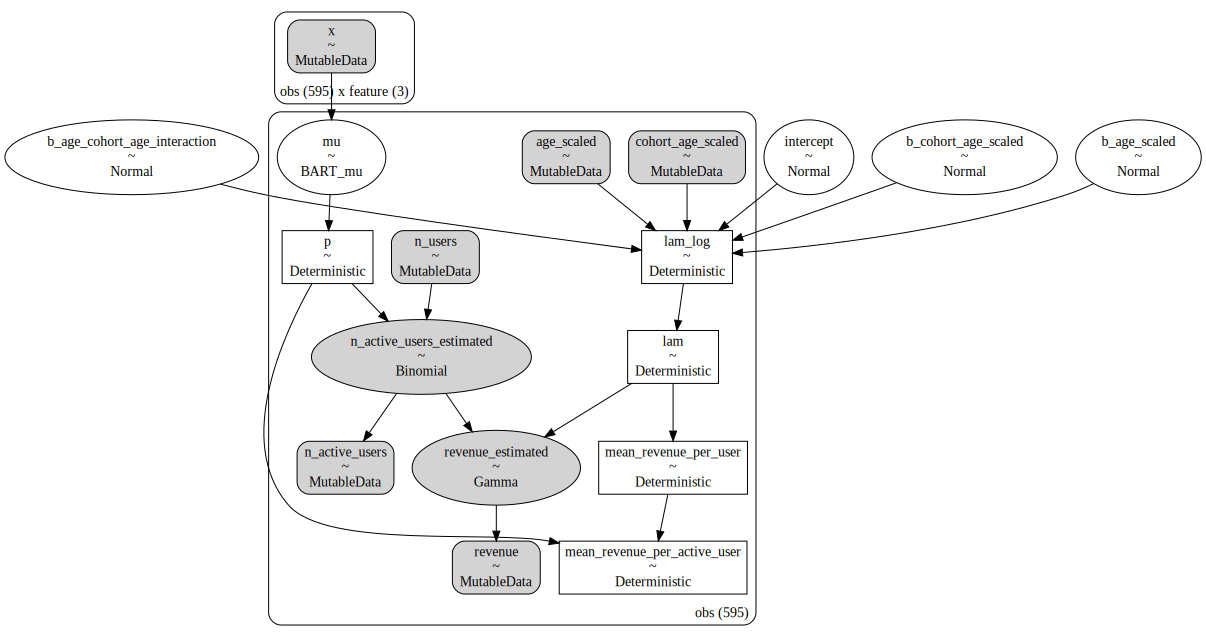
\includegraphics[width=\textwidth]{images/revenue_retention_33_0.png}
    \caption{Cohort-revenue-retention model structure. This diagram illustrates the coupling mechanism that connects
        the two components of our framework. On the left, the retention component models the number of active users
        $N_{\text{active}}$ as a binomial random variable, where the retention probability $p$ is modeled as a function 
        of features including cohort age, age (cohort identifier), and month (seasonality). On the right, the revenue component
        models total revenue as a gamma-distributed random variable, with the shape parameter directly determined by
        $N_{\text{active}}$ from the retention model. This coupling through active users provides a natural connection:
        changes in retention patterns automatically propagate to revenue predictions, ensuring consistency between the two
        metrics while allowing each component to use appropriate distributional assumptions and feature sets.}
    \label{fig:revenue_retention_model}
\end{figure}

Figure \ref{fig:revenue_retention_model} shows the complete model structure in plate notation (common in Bayesian graphical models).

\subsection{Features: Cohort Age and Period}

Before going into the details of modeling the latent variables $p$ and $\lambda$, we define the core features used in the model.
Typical purchase databases contain transactional history at user level. We want an approach general enough to benefit
from the most common features instead of heavy feature engineering. It is natural to consider the following features 
to model the retention and revenue matrices:

\begin{itemize}
    \item {\bf Cohort age}: Age of the cohort in months, representing the time since the cohort was formed.
    \item {\bf Age}: Age of the cohort with respect to the observation time.
          This feature serves as a numerical encoder for the cohort's position in time.
    \item {\bf Month}: Month of the observation time (period), capturing seasonality effects.
\end{itemize}

For example, if our observation month is {\em 2022-11} and we consider the cohort {\em 2022-09}, the age of this cohort
is $2$ months, as the age is always calculated relative to the observation period. This cohort was observed during two
periods: {\em 2022-10} and {\em 2022-11} with cohort ages $1$ and $2$ respectively.

All these features are available for out-of-sample predictions, ensuring model applicability for forecasting.
In practice, additional covariates can be added to the model. The only requirement for out-of-sample predictions is that
these covariates must be available for future observation periods.

\subsection{Flexible Modeling of Latent Variables}

A key strength of our framework is the flexibility in how we model the latent variables $p$ (retention probability) and 
$\lambda$ (revenue rate). The coupling mechanism remains the same regardless of the specific functional forms chosen.

\subsubsection{Retention Probability $p$}

We recommend modeling the retention probability using flexible non-parametric methods that can capture complex 
relationships without requiring explicit specification of functional forms:

\begin{align*}
    \textrm{logit}(p) & = f(\text{cohort age}, \text{age}, \text{month})
\end{align*}

where $f$ can be:

\begin{itemize}
    \item \textbf{BART (Bayesian Additive Regression Trees)}: Our recommended baseline. BART \cite{chipman2010bart} 
          represents the unknown function as a sum of regression trees, automatically learning non-linear 
          relationships and interactions. The PyMC implementation \cite{quiroga2022bart} provides interpretability 
          tools such as partial dependence plots (PDP) and individual conditional expectation (ICE) plots.
    
    \item \textbf{Neural Networks}: For applications requiring fast inference or scaling to very large datasets, 
          neural networks with stochastic variational inference offer an alternative (see Section \ref{sec:alternative_approaches}).
    
    \item \textbf{Linear Models}: For simpler applications or as a baseline comparison, a linear model with 
          interactions can be used.
\end{itemize}

\subsubsection{Revenue Rate $\lambda$}

For the revenue component, we typically find that simpler parametric models suffice:

\begin{align*}
    \log(\lambda) = ( & \text{intercept}                                                                          \\
                      & + \beta_{\text{cohort age}} \times \text{cohort age}                                      \\
                      & + \beta_{\text{age}} \times \text{age}                                                    \\
                      & + \beta_{\text{cohort age} \times \text{age}} \times \text{cohort age} \times \text{age})
\end{align*}

A key insight from both synthetic and real-world applications is that we typically don't need to explicitly
model seasonality in the revenue component, as seasonal patterns are already captured by the retention component
through the coupling mechanism. However, if the business model has a strong seasonal component in average basket sizes, 
an additional seasonal term can be added.

\subsection{Advantages of the Framework}

This modeling strategy offers several distinct advantages:

\begin{itemize}
    \item \textbf{Flexibility in relationship modeling}: The non-parametric approach
          can capture complex non-linear relationships between cohorts, time periods, and behavioral metrics without requiring
          explicit specification of these relationships.

    \item \textbf{Integrated seasonality}: The model naturally incorporates seasonal patterns without requiring separate
          components or preprocessing steps.

    \item \textbf{Extensibility}: Additional covariates (e.g., macroeconomic indicators, marketing campaign intensities, etc.) can
          be seamlessly integrated into the model. The framework also extends naturally to hierarchical multi-market 
          settings (Section \ref{sec:hierarchical}).

    \item \textbf{Uncertainty quantification}: The Bayesian framework provides natural uncertainty estimates around all
          predictions, enabling risk-aware decision making.

    \item \textbf{Information sharing across cohorts}: Newer cohorts with limited historical data benefit from patterns
          learned from more established cohorts.
\end{itemize}

\begin{remark}[Conditioning on Active Users]
    When running inference (MCMC or SVI), we condition on the number of active users $N_{\text{active}}$ rather than
    directly on the observed retention rates. The reason to treat retention as a latent variable is to obtain better uncertainty
    estimates depending on the cohort size ($N_{\text{total}}$) and the number of active users ($N_{\text{active}}$). Recall
    that the standard error of a proportion is $\sqrt{p(1-p)/N_{\text{total}}}$.
\end{remark}

%%%%%%%%%%%%%%%%%%%%%%%%%%%%%%%%%%%%%%%%%%%%%%%%%%%%%%%%%%%%%%%%%%%%%%%%%%%%%%%
% SECTION 4: SYNTHETIC EXAMPLE
%%%%%%%%%%%%%%%%%%%%%%%%%%%%%%%%%%%%%%%%%%%%%%%%%%%%%%%%%%%%%%%%%%%%%%%%%%%%%%%

\section{A Synthetic Example}\label{sec:synthetic_example}

We now instantiate the general framework from Section \ref{sec:model_framework} using synthetic data. While our framework 
has been successfully applied to real business datasets (see Section \ref{sec:hm_application}), we present results using 
synthetic data for reproducibility and to demonstrate the approach under controlled conditions. The synthetic dataset is 
designed to reflect realistic business scenarios, incorporating the types of temporal patterns and cohort dynamics commonly 
observed in practice.

The synthetic dataset is available as a CSV file from \cite{orduz_revenue_retention}, and the code to generate this dataset
deterministically is publicly available in \cite{orduz_revenue_retention_data_code}. This ensures full reproducibility of
our results and allows researchers to explore model behavior under controlled conditions.

\subsection{Exploratory Data Analysis}

Before fitting our model, we conduct exploratory data analysis to understand the key patterns in the data. This analysis
validates our modeling choices and provides a baseline for evaluating model performance. Figure \ref{fig:retention_matrix}
(shown in the Introduction) displays the retention matrix per cohort and period. Two key observations stand out:

\begin{enumerate}
    \item The retention exhibits a clear seasonal pattern with respect to the period, being higher in the last months of the
          year and lower in the middle of the year. This seasonality pattern is more evident in Figure
          \ref{fig:retention_seasonal}.
    \item Retention appears to increase as the cohort age decreases. This trend is apparent when comparing retention values
          for periods in November across different cohort ages.
\end{enumerate}

\begin{figure}
    \centering
    \includegraphics[width=\textwidth]{images/revenue_retention_19_0.png}
    \caption{Retention as a function of the period, demonstrating the yearly seasonality pattern in retention values.}
    \label{fig:retention_seasonal}
\end{figure}

It's important to remember that retention is a ratio, making cohort size an important factor. For instance, a retention rate
of 0.4 could represent either $4/10$ or $4\times 10^{5} / 10^{6}$. The former case carries considerably more uncertainty in
its estimation. This insight motivates the use of the number of active users (rather than the raw rate) in our likelihood, 
as the Binomial distribution naturally accounts for this sample-size-dependent uncertainty. 
As shown in Figure \ref{fig:active_users} (in the Introduction), we observe that more recent cohorts have 
significantly more active users, a pattern we want our model to account for.

Next, we examine revenue patterns. Figure \ref{fig:revenue_matrix} presents revenue by cohort, showing a strong correlation with the
number of active users. This suggests that revenue per user remains relatively stable over time. To verify this, we compute
revenue per user as a function of age and period (Figure \ref{fig:revenue_per_user}) as well as revenue per {\em active} user
(Figure \ref{fig:revenue_per_active_user}). The key difference between these metrics is that revenue per user divides by
total cohort size, while revenue per active user divides by the number of active users in the given period. We observe 
the following for the revenue data\footnote{These types of patterns are actually common in real applications. This synthetic
    dataset is motivated by real applications where the model was proven to be very effective.}:

\begin{itemize}
    \item Revenue per user exhibits a clear seasonality pattern, consistent with the seasonal pattern observed in retention.
    \item Revenue per active user does not show the same seasonality pattern since seasonal effects are already captured in
          the denominator (active users). Additionally, revenue per active user appears to decrease as cohort age increases,
          suggesting that older cohorts generate less revenue per active customer.
\end{itemize}

These exploratory findings validate our modeling strategy. The strong seasonality in retention motivates the inclusion of
month (period) as a feature in the retention component. The heterogeneity across cohort ages suggests that flexible non-parametric
modeling will be valuable for capturing these varying patterns. The relationship between revenue and active users justifies
our coupling mechanism, while the patterns in revenue per active user guide the parametric specification of the revenue
component.

\begin{figure}
    \centering
    \includegraphics[width=\textwidth]{images/revenue_retention_27_0.png}
    \caption{Revenue per user across cohorts. This visualization normalizes the total revenue by the original cohort size,
        showing the average revenue generated per initially acquired user.}
    \label{fig:revenue_per_user}
\end{figure}

\begin{figure}
    \centering
    \includegraphics[width=\textwidth]{images/revenue_retention_25_0.png}
    \caption{Revenue per active user across cohorts. This metric divides total revenue by the number of active users in each
        period, isolating spending patterns from retention effects.}
    \label{fig:revenue_per_active_user}
\end{figure}

\subsection{Model Instantiation}\label{sec:model_instantiation}

For this synthetic example, we instantiate the general framework using BART for the retention component and a linear model 
for the revenue component. This combination represents our recommended baseline.

\subsubsection{Retention Component with BART}

We model the retention probability using BART:

\begin{align*}
    N_{\text{active}} & \sim \text{Binomial}(N_{\text{total}}, p)                  \\
    \textrm{logit}(p) & = \text{BART}(\text{cohort age}, \text{age}, \text{month})
\end{align*}

The BART component models the unknown retention latent variable as a sum of many regression trees, where
each tree contributes a small part to the overall prediction \cite{chipman2010bart}. The key advantage is that this ensemble
automatically learns complex non-linear patterns and interactions without requiring the analyst to specify functional forms.
The prior specification encourages sparse, shallow trees that collectively capture the data structure while avoiding overfitting.

We implement BART using the PyMC framework via \cite{quiroga2022bart}, which handles the technical details of tree structure
priors and parameter estimation. The main tuning parameter is the number of trees $m$. For our retention
modeling, we typically start with $m = 20$ trees and increase incrementally (e.g., to $50$ or $100$) while monitoring posterior
predictive fit. BART is relatively insensitive to this choice for sufficiently large $m$, but smaller values offer
computational efficiency and maintain interpretability through tools like partial dependence plots.
Readers interested in the mathematical details of BART priors—including tree topology priors, splitting rule distributions,
and leaf parameter specifications—are referred to the comprehensive treatment in \cite{chipman2010bart} and the implementation
details in \cite{quiroga2022bart}.

\begin{remark}[Additional Covariates]
    A key advantage of the BART model is its flexibility in incorporating additional covariates. In real business
    applications, we have successfully added customer segmentation features (such as acquisition media channels from
    attribution models). This provides valuable insights into media channel return-on-investment (ROI), allowing businesses
    to consider not just acquisition costs but also estimated customer lifetime value through this combined model.
\end{remark}

\begin{remark}[Baseline Linear Model]
    We always recommend starting with a simple baseline, such as a linear model
    \begin{align*}
        \text{logit}(p)  = & \left(\text{intercept} + \beta_{\text{cohort age}} \times \text{cohort age} + \beta_{\text{age}} \times \text{age} \right.                        \\
                           & \left. + \beta_{\text{cohort age} \times \text{age}} \times \text{cohort age} \times \text{age} + \beta_{\text{month}} \times \text{month}\right)
    \end{align*}

    as described in \cite{orduz_revenue_retention}. In many cases, these baseline models are sufficient for the first
    iteration to get the decision-making process moving forward. Nevertheless, in many real applications, we have seen that
    the BART models can significantly improve the performance of the model (in and out of sample predictions).
\end{remark}

\subsubsection{Revenue Component with Linear Model}

For the revenue component, we employ a gamma random variable $\text{Gamma}(N_{\text{active}}, \lambda)$ (inspired by
\cite{stucchio2015bayesian}). The gamma distribution is a natural choice for modeling revenue as it ensures non-negativity
and provides flexibility in capturing different revenue distributions through its shape and rate parameters. The mean of
this gamma distribution is $N_{\text{active}} / \lambda$, allowing us to interpret $1 / \lambda$ as the {\em average
revenue per active user}. By using $N_{\text{active}}$ as the shape parameter, we ensure that cohorts with more active
users have lower relative variance (coefficient of variation $1/\sqrt{N_{\text{active}}}$), which aligns with the intuition
that aggregated revenue from larger cohorts should be more stable. 

We model $\log(\lambda)$ using a linear function of cohort age, age, and their interaction. As a preprocessing step, we 
standardize these features for the linear model component (we keep the same notation for the variables for simplicity). 
This allows us to specify priors for the regression coefficients in terms of the effect of a one-standard-deviation change 
in the predictor, enabling effective regularization through standard normal priors for the coefficients (see \cite{orduz_retention_bart}).

\begin{align*}
    \text{Revenue}    & \sim \text{Gamma}(N_{\text{active}}, \lambda)                                             \\
    \log(\lambda) = ( & \text{intercept}                                                                          \\
                      & + \beta_{\text{cohort age}} \times \text{cohort age}                                      \\
                      & + \beta_{\text{age}} \times \text{age}                                                    \\
                      & + \beta_{\text{cohort age} \times \text{age}} \times \text{cohort age} \times \text{age})
\end{align*}

\begin{remark}[Cohort Age Encoding]
    The {\em age} feature characterizes each cohort's temporal position. While we could replace this numerical encoding with
    a one-hot encoding of cohorts and add hierarchical structure to pool information across cohorts, the numerical encoding
    is more parsimonious under the assumption that temporally proximate cohorts behave more similarly than distant ones.
\end{remark}

\subsubsection{Complete Model Specification with Priors}

In summary, for this synthetic example, the cohort-revenue-retention model is specified as:

\begin{align*}
    \text{Revenue}                              & \sim \text{Gamma}(N_{\text{active}}, \lambda)                                             \\
    \log(\lambda) = (                           & \text{intercept}                                                                          \\
                                                & + \beta_{\text{cohort age}} \times \text{cohort age}                                      \\
                                                & + \beta_{\text{age}} \times \text{age}                                                    \\
                                                & + \beta_{\text{cohort age} \times \text{age}} \times \text{cohort age} \times \text{age}) \\
    N_{\text{active}}                           & \sim \text{Binomial}(N_{\text{total}}, p)                                                 \\
    \textrm{logit}(p)                           & = \text{BART}(\text{cohort age}, \text{age}, \text{month})                                \\
    \text{intercept}                            & \sim \text{Normal}(0, 1)                                                                  \\
    \beta_{\text{cohort age}}                   & \sim \text{Normal}(0, 1)                                                                  \\
    \beta_{\text{age}}                          & \sim \text{Normal}(0, 1)                                                                  \\
    \beta_{\text{cohort age} \times \text{age}} & \sim \text{Normal}(0, 1)
\end{align*}

\subsection{Model Fitting and Diagnostics}

With the model fully specified, we implement and fit it using PyMC \cite{pymc2023}, leveraging the BART implementation
from \cite{quiroga2022bart}. Complete implementation details and code are available in \cite{orduz_revenue_retention}, where
we follow the {\em Bayesian workflow} (\cite{gelman2020bayesianworkflow}). After fitting the model using MCMC, we conduct 
thorough diagnostics to ensure reliable inference. 

Figure \ref{fig:posterior_predictive} presents a critical diagnostic: the posterior predictive distribution for both model
components. These plots compare the distribution of observed values against the distribution of values simulated from the
fitted model's posterior predictive distribution. Close agreement between these distributions indicates that the model
successfully captures the data-generating process. For both retention and revenue components, we observe excellent agreement,
with the simulated distributions (red) closely matching the observed distributions (black). This suggests the model
provides an adequate fit to the data. 

Beyond the posterior predictive check, we examine convergence diagnostics for
the model parameters. Figure \ref{fig:trace} displays trace plots for the linear model parameters
(intercept and regression coefficients). These plots show the evolution of parameter values across MCMC iterations for each chain.
Good mixing—evidenced by chains that explore the parameter space efficiently without getting stuck—is essential for reliable inference.
We observe healthy mixing for all parameters, with no divergences or convergence warnings. All $\hat{R}$ statistics are below $1.01$,
confirming convergence. These diagnostics give us confidence that the MCMC sampling has successfully explored the posterior
distribution and that our parameter estimates are reliable.

\begin{figure}
    \centering
    \includegraphics[width=\textwidth]{images/revenue_retention_37_0.png}
    \caption{Posterior predictive distribution of the retention (left) and revenue (right) components, showing good fit to
        the observed data. These cumulative density plots compare the distributions of observed values (black) with simulated
        values from the posterior predictive distribution (orange), providing a visual assessment of model fit.}
    \label{fig:posterior_predictive}
\end{figure}

\begin{figure}
    \centering
    \includegraphics[width=\textwidth]{images/revenue_retention_41_0.png}
    \caption{Trace plots for the linear model parameters, showing good mixing and convergence of the MCMC chains.}
    \label{fig:trace}
\end{figure}

\subsection{Variable Importance}

A key advantage of using BART over more opaque machine learning methods is the availability of tools for understanding which
features drive predictions and how they influence outcomes. The BART implementation in \cite{quiroga2022bart} provides
interpretability tools that allow us to peer inside the model and extract actionable insights about retention drivers.
Figure \ref{fig:ice_plot} presents {\em Partial Dependence Plot (PDP)} and {\em Individual Conditional Expectation (ICE)} plots for the
retention component. These visualization techniques reveal how the model's predictions change as each feature varies
while holding all other features constant. Each line represents a different observation from the dataset, showing how the
predicted retention probability would change for that observation if we modified only the feature of interest. The solid line
represents the PDP plot, which is the average of the ICE plots. These plots allow us to understand how the retention probability varies
for different values of the features and reveals potential non-linear relationships or interaction effects that might not
be apparent in aggregate statistics. \\

\begin{figure}
    \centering
    \includegraphics[width=\textwidth]{images/retention_bart_32_1.png}
    \caption{PDP (solid line) and ICE (dashed lines) plots for the retention component.}
    \label{fig:ice_plot}
\end{figure}

In this specific example, we can extract the following insights:

\begin{itemize}
    \item The ICE plots show how the retention rate decreases with both cohort age and age. This is not surprising as we saw in the exploratory data analysis.
    \item We see that the ICE plots have a similar trend to the PDP plots. This hints that the interaction effects are
          not so important in this case. This is also something we saw in the linear model where the interaction coefficient
          was relatively small (see \cite{orduz_retention}).
    \item We clearly see the seasonality component of the PDP / ICE plots resemble the regression coefficients in the linear
          model from \cite{orduz_retention}. This is simply representing the strong seasonal component of the data.
\end{itemize}

In addition, we can extract a relative importance for the different features using the contribution to the in-sample $R^2$,
as shown in Figure \ref{fig:variable_importance}.

\begin{figure}
    \centering
    \includegraphics[width=\textwidth]{images/retention_bart_32_0.png}
    \caption{Variable importance for the retention component based on the in-sample $R^2$.}
    \label{fig:variable_importance}
\end{figure}

These types of plots are very valuable to understand the {\em drivers} of the retention component.

\subsection{Predictions}\label{sec:predictions}

Having established that our model fits the data well and that MCMC sampling has converged, we now examine the model's
predictive performance. This section evaluates predictions in two contexts: in-sample predictions that assess how well the
model captures observed patterns, and out-of-sample predictions that test the model's ability to forecast future retention
and revenue for periods beyond the training data.

\subsubsection{In-Sample Predictions}

We first evaluate the model's in-sample performance by comparing the posterior predictive mean against the observed values.
Figure \ref{fig:in_sample_mean} shows the comparison for both retention and revenue components, with points closer to the
diagonal line indicating better fit. Beyond point estimates, we can visualize the full posterior predictive distribution
to assess model uncertainty. Figure \ref{fig:in_sample_retention} shows the posterior predictive distribution of retention
for selected cohorts, with $94\%$ HDI (Highest Density Interval). Note how the intervals are narrower for more recent
cohorts with more data, reflecting greater certainty in these predictions. Overall, the predictions effectively capture the
observed retention patterns, including seasonality. For the revenue component, Figure \ref{fig:in_sample_revenue} shows
the posterior predictive distribution compared to actual revenue values. The model successfully captures the revenue
variability across different cohorts and time periods. We can use the whole posterior distribution to make custom visualizations
of quantities of interests like the revenue per active user, as shown in Figure \ref{fig:additional_predictions}.

\begin{figure}
    \centering
    \begin{tabular}{cc}
        \includegraphics[width=0.5 \textwidth]{images/revenue_retention_45_0.png} &
        \includegraphics[width=0.5 \textwidth]{images/revenue_retention_47_0.png}
    \end{tabular}
    \caption{Retention (left) and revenue (right) in-sample posterior predictive mean values plotted against the actual
        observations. These scatter plots provide a quantitative assessment of model fit by comparing predicted
        versus observed values, with points closer to the diagonal line indicating better predictions.}
    \label{fig:in_sample_mean}
\end{figure}

\begin{figure}
    \centering
    \includegraphics[width=\textwidth]{images/revenue_retention_51_0.png}
    \caption{Retention in-sample posterior predictive distribution for selected cohorts, showing $94\%$ HDI (blue shaded areas)
        and observed retention values (blue points). This visualization displays the model's predictive performance for
        retention across time for different cohorts, with uncertainty quantified through highest density intervals.
        The narrower intervals for more recent cohorts (bottom panels) reflect greater certainty due to more available
        data, while the consistent capture of observed values within the intervals indicates well-calibrated uncertainty
        estimates. The plots also reveal the model's ability to adapt to cohort-specific patterns and seasonal
        fluctuations, demonstrating its flexibility in capturing complex temporal dynamics.}
    \label{fig:in_sample_retention}
\end{figure}

\begin{figure}
    \centering
    \includegraphics[width=\textwidth]{images/revenue_retention_53_0.png}
    \caption{Revenue in-sample posterior predictive distribution for selected cohorts, showing $94\%$ HDI (blue shaded areas)
        and observed revenue values (blue points). These plots illustrate the model's revenue predictions and associated
        uncertainty across time for different cohorts. The successful capture of observed values within the HDI bands
        demonstrates the model's ability to accurately represent not just central tendencies but also the inherent
        variability in revenue. The visualization highlights how our coupled modeling approach effectively propagates
        uncertainty from the retention component to revenue estimates, providing business stakeholders with realistic
        confidence intervals for financial planning and analysis.}
    \label{fig:in_sample_revenue}
\end{figure}

\begin{figure}
    \includegraphics[width=\textwidth]{images/revenue_retention_56_0.png}
    \caption{Additional view of posterior predictions across cohorts, illustrating the model's ability to capture
        cohort-specific patterns. This panel view organizes predictions by cohort (columns) and shows how the model
        adapts to the unique characteristics of each customer group.}
    \label{fig:additional_predictions}
\end{figure}

\subsubsection{Out-of-Sample Predictions}

The true test of any predictive model is its performance on unseen data. We evaluate our model's forecasting capabilities
using a holdout set consisting of data after {\em 2022-11}, which was not used during model training. Figures
\ref{fig:out_sample_retention} and \ref{fig:out_sample_revenue} show the out-of-sample predictions for retention and
revenue, respectively. The vertical dashed lines indicate the train/test split point. Several key observations emerge:

\begin{enumerate}
    \item The model successfully predicts both retention and revenue patterns for future periods, with most actual
          observations falling within the $94\%$ HDI.

    \item The model effectively captures the seasonal patterns in retention, correctly predicting the expected peaks and
          troughs in future months based on historical patterns.

    \item For newer cohorts with limited training data (e.g., the {\em 2022-07} cohort with only 4 data points in
          training), the model still produces reasonable predictions by leveraging information learned from older cohorts.
          This demonstrates effective transfer of knowledge across cohorts.

    \item The $94\%$ HDI appropriately widens for more distant future predictions, reflecting increasing uncertainty as we
          forecast further ahead. \\
\end{enumerate}

\begin{figure}
    \centering
    \includegraphics[width=\textwidth]{images/revenue_retention_66_0.png}
    \caption{Retention out-of-sample posterior predictive distribution for (random) selected cohorts.}
    \label{fig:out_sample_retention}
\end{figure}

\begin{figure}
    \centering
    \includegraphics[width=\textwidth]{images/revenue_retention_68_0.png}
    \caption{Revenue out-of-sample posterior predictive distribution for (random) selected cohorts.}
    \label{fig:out_sample_revenue}
\end{figure}

These results highlight one of the key advantages of our Bayesian approach: the ability to make probabilistic forecasts with
well-calibrated uncertainty using highest density intervals (HDI). The model provides not just point estimates but complete
distributions, allowing businesses to understand the range of possible outcomes and make risk-aware decisions. The effective
transfer of information across cohorts is particularly valuable for new cohorts where limited data is available.

\section{Alternative Non-Parametric Approaches}\label{sec:alternative_approaches}

The framework we have presented centers on BART for the retention component, a choice motivated by BART's flexibility,
interpretability through PDP/ICE plots, and relatively straightforward hyperparameter tuning. However, the modular nature
of our approach means the BART component can be replaced with other flexible function approximators. In this section, we
briefly discuss one particularly promising alternative: neural networks with Bayesian inference. This discussion serves two
purposes: first, it demonstrates the framework's flexibility and extensibility; second, it provides practitioners with
guidance on when alternative implementations might be preferable.

While Bayesian Additive Regression Trees provide a powerful non-parametric approach for modeling the retention component,
neural networks coupled with efficient Bayesian inference techniques offer an alternative that combines flexibility with
computational efficiency, albeit with some tradeoffs in interpretability.

\subsection{Neural Networks with NumPyro}

As demonstrated by \cite{orduz_revenue_retention_numpyro}, the BART component in our model can be replaced with a neural
network implemented using Flax (\cite{flax2020github}), with inference performed using NumPyro (\cite{phan2019composable}). The modified model
structure becomes:

\begin{align*}
    \text{Revenue}    & \sim \text{Gamma}(N_{\text{active}}, \lambda)                                             \\
    \log(\lambda) = ( & \text{intercept}                                                                          \\
                      & + \beta_{\text{cohort age}} \times \text{cohort age}                                      \\
                      & + \beta_{\text{age}} \times \text{age}                                                    \\
                      & + \beta_{\text{cohort age} \times \text{age}} \times \text{cohort age} \times \text{age}) \\
    N_{\text{active}} & \sim \text{Binomial}(N_{\text{total}}, p)                                                 \\
    \textrm{logit}(p) & = \text{NN}(\text{cohort age}, \text{age}, \text{month})
\end{align*}

where $\text{NN}$ represents a neural network. Even a simple architecture with one hidden layer containing just $4$ units and
sigmoid activation functions can capture the complex patterns in retention data effectively.

\subsection{Advantages of the Neural Network Approach}

This neural network approach offers several advantages:

\begin{enumerate}
    \item \textbf{Computational efficiency}: Inference can be performed using stochastic variational inference (SVI), which
          is significantly faster than the MCMC sampling required for BART models. This enables rapid model iteration and
          scaling to larger datasets.

    \item \textbf{Flexibility in inference methods}: Beyond SVI, the NumPyro framework allows for various sampling methods,
          including NUTS (No U-Turn Sampler) for full Bayesian inference when needed, as well as integration with other
          JAX-based probabilistic programming tools like BlackJax (\cite{cabezas2024blackjax}). To be fair, this can
          also be done with PyMC thanks to the PyTensor backend.

    \item \textbf{Comparable predictive performance}: Experiments on the same synthetic dataset show that the neural network
          approach produces similar retention and revenue predictions as the BART-based model, with well-calibrated $94\%$ HDIs
          that appropriately capture uncertainty.

    \item \textbf{Development workflow}: The computational efficiency enables an iterative workflow where initial model
          development and testing can use fast SVI methods, with final inference performed using full MCMC sampling if desired.
\end{enumerate}

\subsection{Limitations of Neural Networks Compared to BART}

Despite these advantages, the neural network approach does have some limitations when compared to BART:

\begin{enumerate}
    \item \textbf{Reduced interpretability}: Unlike BART, neural networks do not naturally provide partial dependence plots
          (PDP) or individual conditional expectation (ICE) plots. These visualizations, which help understand how individual
          predictors affect the target variable, require additional custom implementation with neural networks.

    \item \textbf{Architecture selection}: Neural networks require specification of the network architecture (number of
          layers, units per layer, activation functions), which introduces additional hyperparameters that must be selected,
          whereas BART requires fewer tuning decisions.
\end{enumerate}

\subsection{Practical Considerations}

The choice between BART and neural network approaches depends on the specific needs of the application:

\begin{itemize}
    \item For applications where interpretability is paramount and computational efficiency is less critical, BART may be
          preferred.

    \item For large-scale applications where inference speed is essential or when rapid model iteration is needed, the neural
          network approach with SVI offers significant advantages.

    \item In some cases, a hybrid approach might be valuable—using the faster neural network model for initial exploration
          and prototyping, then moving to BART for final analysis when interpretability is needed.
\end{itemize}

The implementation details and complete code examples for the neural network approach can be found in
\cite{orduz_revenue_retention_numpyro}.

\section{Extension to Hierarchical Multi-Market Modeling}\label{sec:hierarchical}

\subsection{Motivation and Approach}

Organizations operating across multiple markets or customer segments frequently encounter an asymmetry in data
availability: some markets are mature with extensive cohort histories, while others are nascent with only a few observed
cohorts. Modeling each market independently wastes valuable information that could be shared across markets, while complete
pooling ignores market-specific dynamics. A hierarchical structure provides an elegant solution to this challenge by enabling
information pooling while preserving market-specific patterns.

The business motivation for hierarchical modeling is compelling. Consider a company expanding into new geographic regions or
launching products in new market segments. Early-stage markets lack the data needed for reliable independent forecasts, yet
business decisions—resource allocation, growth projections, strategic planning—cannot wait years for sufficient data
accumulation. By borrowing information from more established markets through hierarchical priors, we can generate credible
forecasts for young markets that would otherwise be impossible to model reliably. \\

We extend the neural network approach from Section \ref{sec:alternative_approaches} to accommodate multiple markets through two key modifications:

\begin{itemize}
    \item \textbf{Retention component}: We incorporate market identity as an additional feature in the neural network. The
          network learns market-specific retention patterns while sharing information about temporal dynamics (cohort age,
          calendar effects, seasonality) across markets.

    \item \textbf{Revenue component}: We implement a hierarchical linear model where market-specific regression coefficients
          are drawn from common hierarchical priors. This allows each market to have its own revenue dynamics while constraining
          these parameters to be similar across markets through the prior distribution.
\end{itemize}

The hierarchical structure naturally addresses the data asymmetry problem: markets with abundant data inform the hierarchical
priors, which in turn regularize predictions for data-sparse markets toward sensible values. Crucially, the coupling mechanism
between retention and revenue components remains intact in this hierarchical setting—the number of active users predicted by
the retention model still informs the revenue model's shape parameter.

\subsection{Synthetic Multi-Market Data}

To demonstrate the hierarchical extension, we extend our synthetic data generation process to create cohort-level observations
across four markets with varying maturity levels (recall we train until November $2022$ in the synthetic data generation process)\footnote{
    The code to generate the synthetic data is also available in \cite{orduz_revenue_retention_data_code} to ensure reproducibility.
}:

\begin{itemize}
    \item \textbf{Market A}: Starting from January $2020$ (mature, most data)
    \item \textbf{Market B}: Starting from February $2021$ (moderately mature)
    \item \textbf{Market C}: Starting from January $2022$ (developing)
    \item \textbf{Market D}: Starting from July $2022$ (youngest)
\end{itemize}

The data generation process maintains the same retention and revenue dynamics described in Section \ref{sec:synthetic_example}, but now each market has
its own data realization. We apply the same train/test split strategy, holding out the most recent periods for validation.
Figure \ref{fig:hierarchical_data} visualizes the data structure, showing cohort availability and revenue patterns across the
four markets.

\begin{figure}[H]
    \centering
    \includegraphics[width=\textwidth]{images/hierarchical_revenue_retention_13_2.png}
    \caption{Retention matrix for Market $C$. We just have $10$ cohorts of data available for this market.}
    \label{fig:hierarchical_data}
\end{figure}

This multi-market setup creates a realistic challenge: can we forecast revenue for Market $C$, which has limited data,
by leveraging patterns learned from Markets $A$, $B$, and $D$?

\subsection{Results and Information Pooling}

The hierarchical model achieves strong predictive performance across all markets. Figure \ref{fig:hierarchical_predictions}
shows revenue predictions for Market $C$ by leveraging patterns learned from Markets $A$, $B$, and $D$, demonstrating that the
model successfully borrows strength from more mature markets to generate accurate forecasts despite having only $10$ cohorts
and less of a year of data.

\begin{figure}[H]
    \centering
    \includegraphics[width=\textwidth]{images/hierarchical_revenue_retention_75_0.png}
    \caption{Revenue predictions for four selected cohorts in Market $C$.}
    \label{fig:hierarchical_predictions}
\end{figure}

Several key findings emerge from the hierarchical implementation:

\begin{itemize}
    \item \textbf{Successful information pooling}: Market $C$ achieves prediction accuracy that would be impossible with
          independent modeling. Note that the forecast contains the seasonal component, which would be impossible to capture
          with a single model on Market $C$ as we do not even have a complete year of data.
          The hierarchical priors effectively transfer knowledge about retention decay patterns and revenue
          dynamics from mature markets.

    \item \textbf{Market-specific adaptation}: While borrowing information, the model still captures market-specific patterns.
          Each market's predictions reflect its own data when available, rather than being dominated by the larger markets.

    \item \textbf{Appropriate uncertainty quantification}: The highest density intervals are wider for Market $C$ than for more
          established markets (e.g. Market $A$, for which the results look almost the same as in Section \ref{sec:synthetic_example}),
          correctly reflecting the greater uncertainty due to limited data. This honest uncertainty quantification is crucial
          for business decision-making.

    \item \textbf{Coupling mechanism preserved}: The connection between retention and revenue components functions effectively in
          the hierarchical setting. Active user predictions from the retention model inform revenue forecasts across all markets.
\end{itemize}

The hierarchical extension demonstrates that the framework's core architecture—the coupling between retention and revenue—
naturally extends to more complex settings. This extensibility is not accidental but rather a consequence of the modular
design: the coupling mechanism operates at the cohort-observation level and is agnostic to whether those observations come from
a single market or multiple markets with hierarchical structure.

\subsection{Implementation Notes}

For computational efficiency with multiple markets, we implement the hierarchical model using SVI in NumPyro rather than MCMC sampling.
SVI provides approximate posterior distributions through optimization, enabling the model to scale to tens or hundreds of markets
where full MCMC would be computationally prohibitive\footnote{
    SVI is knows to underestimate the uncertainty, but it is still a valid approximation for the posterior distribution.
}. For applications with fewer markets (say, $5-10$), MCMC remains a viable
alternative that may provide more accurate uncertainty quantification. The complete implementation, including data generation,
model specification, and visualization code, is available at \cite{orduz_hierarchical_revenue_retention}.
The implementation demonstrates that extending the base framework to hierarchical structures requires modest additional
complexity—primarily the specification of hierarchical priors and the inclusion of market
identifiers in the feature set. That being said, inference on hierarchical models is in general more challenging becuase of the
non-linear geometry of the parameter space. Fortunately, NumPyro offers automatic mechanism to reparameterize the model
to make it more amenable to SVI (\cite{gorinova2020automatic}).

\section{A Real-Dataset Application: The H\&M Transactions Dataset}\label{sec:hm_application}

Having demonstrated our framework on synthetic data with known ground truth, we now validate its practical applicability
using a large-scale real-world dataset.
We apply our cohort-revenue-retention model to the H\&M Personalized Fashion Recommendations dataset \cite{hm_kaggle2022},
a publicly available dataset from a Kaggle competition containing transaction records from the H\&M retail chain.
This dataset provides an excellent testbed for our methodology due to its scale, temporal coverage, and the presence
of realistic patterns in customer purchasing behavior.
The dataset contains approximately $31$ million transactions from over $1.36$ million unique customers, spanning
from September $2018$ to September $2020$. For our cohort analysis, we aggregate customers into monthly cohorts based
on their first purchase date, resulting in $20$ cohorts from November $2018$ to June $2020$. We use a train/test split
at May $2020$, holding out $3$ months of data (June--August 2020) for out-of-sample evaluation. This split allows us
to assess the model's forecasting ability while ensuring sufficient training data for each cohort.
Figures \ref{fig:hm_retention_matrix} and \ref{fig:hm_revenue_matrix} present the retention and revenue matrices
for the H\&M dataset. Several patterns emerge that are characteristic of real retail data:

\begin{itemize}
    \item Retention rates show a clear decay pattern as cohort age increases, with the steepest decline occurring
          in the first few months after customer acquisition.
    \item Revenue patterns closely track the number of active users, consistent with our modeling assumption that
          revenue can be decomposed into active user counts and revenue per active user.
\end{itemize}

\begin{figure}[H]
    \centering
    \includegraphics[width=\textwidth]{images/hm-transactions_16_0.png}
    \caption{Retention matrix for the H\&M dataset (training period).}
    \label{fig:hm_retention_matrix}
\end{figure}

\begin{figure}[H]
    \centering
    \includegraphics[width=\textwidth]{images/hm-transactions_17_0.png}
        \caption{Revenue matrix for the H\&M dataset (training period).}
    \label{fig:hm_revenue_matrix}
\end{figure}

We benchmark our Bayesian cohort-revenue-retention model against three established approaches commonly used for time series
forecasting in business contexts (using two established data science libraries: the Nixtla forecasting framework \cite{nixtla} and the
\texttt{scikit-learn} library \cite{scikit-learn}):\footnote{The notebook to reproduce the benchmark results is available at \url{https://github.com/juanitorduz/website_projects/blob/master/Python/cohort-revenue-retention/hm-transactions.ipynb}.}

\begin{enumerate}
    \item \textbf{AutoMFLES}: An automated multiple seasonal-trend decomposition model from the `StatsForecast` library
          that automatically detects and models multiple seasonalities.
    \item \textbf{Simple Exponential Smoothing (SES)}: A classical time series method that produces forecasts as
          weighted averages of past observations, with weights decaying exponentially.
    \item \textbf{HistGradientBoostingRegressor}: A gradient boosting machine learning model from `scikit-learn`,
          representing modern ML approaches to time series forecasting.
\end{enumerate}

These baselines represent the spectrum of approaches typically considered for cohort-level revenue forecasting.

\begin{figure}[H]
    \centering
    \includegraphics[width=\textwidth]{images/hm-transactions_64_0.png}
    \caption{Revenue predictions comparing the Bayesian model against other benchmark approaches for a selected set of cohorts.}
    \label{fig:hm_revenue_predictions}
\end{figure}


Figure \ref{fig:hm_revenue_predictions} shows revenue predictions for selected cohorts for the Bayesian cohort-revenue-retention model
against the other benchmark model. One can clearly see that the Bayesian model is able to capture the dynamics with well-calibrated 
$94\%$ highest density intervals, while the other benchmark models fail to efficiently use the data to generate accurate predictions.
The reason is that the coupling between retention and revenue provides
key signals to the revenue model that are hard to get from the revenue data, even if we allow arbitrary non-linear relationships
such that the gradient boosting model \texttt{HistGradientBoostingRegressor} can learn.
The failure of other benchmark methods is particularly pronounced for cohorts with limited training history (e.g., the
March $2020$ and April $2020$ cohorts, which have only $2$--$3$ observations before the test period). These methods
cannot extrapolate meaningful patterns from such sparse data. Our framework, by contrast, leverages the shared
structure across all cohorts, learning that retention decays with cohort age, that revenue correlates with active
users, and that seasonal patterns affect all cohorts similarly—to generate reliable predictions even for data-sparse
cohorts. Table \ref{tab:hm_metrics} presents quantitative evaluation metrics comparing out-of-sample prediction accuracy
across all models. We report Mean Absolute Error (MAE), Root Mean Squared Error (RMSE), and Mean Absolute
Percentage Error (MAPE) computed on the held-out test set.

\begin{table}[H]
    \centering
    \caption{Out-of-sample evaluation metrics for revenue prediction on the H\&M dataset. Lower values indicate
        better predictive performance. The Bayesian model substantially outperforms all other approaches.}
    \label{tab:hm_metrics}
    \begin{tabular}{lccc}
        \hline
        \textbf{Model}                & \textbf{MAE} & \textbf{RMSE} & \textbf{MAPE (\%)} \\
        \hline
        Bayesian (BART)               & 97.70        & 169.64        & 10.77              \\
        AutoMFLES                     & 212.61       & 297.81        & 28.07              \\
        SES                           & 157.92       & 230.42        & 17.14              \\
        HistGradientBoostingRegressor & 204.51       & 282.49        & 31.63              \\
        \hline
    \end{tabular}
\end{table}

The quantitative results confirm what the visual comparisons suggest: our Bayesian cohort-revenue-retention model
dramatically outperforms standard time series and machine learning approaches. The improvement is most pronounced
in MAPE, where the Bayesian model achieves $10.77\%$ compared to $17.14\%$--$31.63\%$ for the baselines, reflecting
the model's ability to maintain proportionally accurate predictions across cohorts of varying sizes and revenue
magnitudes. The MAE and RMSE metrics tell a similar story: the Bayesian model's MAE of $97.70$ is roughly half
that of the best-performing baseline (SES at $157.92$), demonstrating substantial improvements in absolute
prediction accuracy.

Finally, Figure \ref{fig:hm_total_revenue} aggregates predictions across all training cohorts to show total revenue forecasting
performance. The Bayesian model's predictions (with $50\%$ and $94\%$ HDI bands) track the actual revenue trajectory,
while baseline methods diverge substantially in the test period.

\begin{figure}[H]
    \centering
    \includegraphics[width=\textwidth]{images/hm-transactions_65_0.png}
    \caption{Total revenue predictions (aggregated across all training cohorts) comparing the Bayesian model with
        baselines. The black line shows observed total revenue, while colored lines show model predictions. The
        Bayesian model's uncertainty bands (blue/orange shading for train/test periods) appropriately capture
        the observed values, while point forecasts from baseline methods miss the actual revenue trajectory.}
    \label{fig:hm_total_revenue}
\end{figure}

\begin{remark}
It is worth noting that individual-level probabilistic models, such as the Shifted Beta Geometric (sBG) model
\cite{FaderHardie2007} implemented in PyMC-Marketing \cite{pymc_marketing}, provide an alternative framework
for modeling customer retention in contractual settings. However, fitting such models using MCMC on datasets
of this scale—with over $1.36$ million unique customers and $31$ million transactions is computationally
prohibitive without substantial investment in specialized hardware infrastructure (e.g., high-end GPUs).
While stochastic variational inference can improve scalability, the cohort-level approach presented in this
paper offers a practical and effective alternative: by aggregating to the cohort level, we dramatically
reduce the computational burden while retaining the ability to capture complex temporal patterns and
provide well-calibrated uncertainty estimates. The benchmark results above demonstrate that this
cohort-level framework not only scales gracefully but also delivers superior predictive performance
compared to standard time series and machine learning baselines.
\end{remark}

\subsection{Comparison with Classical CLV Models}\label{sec:clv_comparison}

To provide a comprehensive evaluation of our proposed framework, we compare it against classical buy-till-you-die (BTYD)
models from the customer lifetime value literature. Specifically, we implement the BG/NBD model \cite{FaderHardie2005}
for modeling purchase frequency and dropout, combined with the Gamma-Gamma model \cite{fader2005rfm} for monetary value
estimation. These models represent the standard approach for CLV estimation in non-contractual settings and are
implemented in PyMC-Marketing \cite{pymc_marketing}\footnote{The complete implementation code for this comparison
is available at \url{https://github.com/juanitorduz/website_projects/blob/master/Python/cohort-revenue-retention/hm-pymc-marketing.ipynb}.}.

\subsubsection{Cohort-Based Fitting Approach}

A key challenge when applying BG/NBD models to retail datasets is their assumption of stationary purchase rates.
The model assumes that each customer's underlying transaction rate remains constant over time, which conflicts
with the strong seasonal patterns observed in fashion retail data. The H\&M dataset exhibits clear seasonality
in both retention and revenue (as shown in Figures \ref{fig:hm_retention_matrix} and \ref{fig:hm_revenue_matrix}),
making a single global BG/NBD model inappropriate.

To address this limitation, we adopt a cohort-based fitting strategy: instead of fitting a single model to all
$1.36$ million customers, we fit separate BG/NBD and Gamma-Gamma model pairs for each of the $20$ monthly cohorts.
This approach implicitly captures some seasonal effects by allowing each cohort to have its own parameter estimates,
reflecting the purchasing patterns of customers acquired during different times of the year. We use maximum a
posteriori (MAP) estimation because full MCMC sampling at this scale, with over one million customers, is
computationally infeasible in practice. Moreover, given the model's inherent limitations (stationarity assumption,
lack of seasonality flexibility), investing substantial computational resources in full Bayesian inference would
not address the fundamental modeling constraints.

\subsubsection{Implementation Challenges and Solutions}

Fitting BG/NBD models via MAP estimation proved challenging for several cohorts with extreme data characteristics.
The optimizer can produce NaN parameter estimates when cohorts exhibit:

\begin{itemize}
    \item \textbf{High repeat rates} ($>90\%$): The optimizer pushes the dropout parameters ($a$ and $b$ in the
          Beta distribution governing dropout probability) toward extreme values, causing numerical instability.
    \item \textbf{Low recency/T ratios} ($<0.25$): Customers who made their last purchase long before the
          observation end appear ``dormant,'' leading to extreme estimates for the dropout shape parameter.
\end{itemize}

To address these convergence issues, we implemented a progressive prior tightening strategy with three tiers
of increasingly informative priors:

\begin{enumerate}
    \item \textbf{Default priors} ($\sigma = 5$): Moderately informative HalfNormal priors that work for
          typical cohorts with balanced repeat rates.
    \item \textbf{Tight priors} ($\sigma = 2$): Used as a fallback for cohorts with high-frequency customers
          (mean frequency $> 20$), constraining the parameter space to avoid extreme values.
    \item \textbf{Very tight priors} ($\sigma = 1$): A final fallback for cohorts with low recency/T ratios,
          strongly constraining parameters near typical values.
\end{enumerate}

The fitting algorithm attempts each configuration in sequence, with multiple random seeds per configuration,
until a valid (non-NaN) fit is obtained. This strategy successfully fitted all $20$ cohorts, though we note
the trade-off: tighter priors stabilize MAP estimation but may introduce bias in parameter estimates.

\subsubsection{Results and Discussion}

Figure \ref{fig:cohort_bg_nbd} presents the revenue predictions from the cohort-based BG/NBD + Gamma-Gamma
models for the same cohorts shown in Figure \ref{fig:hm_revenue_predictions}. Several qualitative observations
emerge from comparing this approach with our BART-based framework:

\begin{figure}[H]
    \centering
    \includegraphics[width=\textwidth]{images/cohort_bg_nbd.png}
    \caption{Revenue predictions using cohort-based BG/NBD + Gamma-Gamma models for selected cohorts.
        Blue lines show observed training revenue, orange lines show model predictions, and orange dots
        indicate observed test revenue.}
    \label{fig:cohort_bg_nbd}
\end{figure}

\begin{itemize}
    \item \textbf{Flat predictions}: The BG/NBD predictions are essentially flat across the test period due to
          the stationarity assumption, unable to capture seasonal patterns visible in the actual data.
    \item \textbf{No cross-cohort information sharing}: Each cohort's model is fitted independently, which is
          particularly problematic for young cohorts with limited training data.
\end{itemize}

Classical BTYD models remain valuable tools for individual-level CLV estimation in stationary settings.
However, for cohort-level and aggregate revenue forecasting, the focus of this paper, our framework offers
practical advantages: it is more accurate for seasonal data, simpler to implement (a single model versus
$20$ separate model pairs), and more interpretable through tools like partial dependence plots. The ability
to naturally incorporate calendar effects and share information across cohorts makes it well-suited for
the business decision-making contexts we target. We could of course think about a fully Bayesian 
hierarchical model where we pool in the parameters of the BG/NBD and Gamma-Gamma models across cohorts,
but this would be computationally prohibitive for the scale of the dataset (which is not uncommon for many businesses).

\subsection{Limitations and Future Work}\label{sec:limitations}

While the proposed framework offers significant advantages in terms of flexibility and predictive accuracy, it is 
important to acknowledge its limitations and potential areas for future development.

First, by operating at the cohort level, the model necessarily sacrifices individual-level granularity. While this 
aggregation reduces noise and improves computational efficiency, it also means that specific customer-level behaviors—such 
as individual product preferences or idiosyncratic purchase triggers—are not explicitly captured. For applications 
requiring highly personalized interventions, this framework should be seen as a complement to, rather than a replacement 
for, individual-level models.

Second, the current coupling mechanism assumes that the average revenue per active user follows a relatively stable 
functional form $\lambda(x)$. While we demonstrated that this holds well in both synthetic and real-world datasets, 
sudden structural breaks in the market (e.g., major policy changes or black-swan events) might require more complex 
modeling of the revenue rate, potentially including stochastic volatility components.

Third, the framework's performance on extremely sparse cohorts remains an area for further investigation. While 
hierarchical information pooling significantly improves predictions for young cohorts, there is a fundamental lower 
bound on the amount of data required to distinguish between different latent drivers. Future work could explore 
incorporating even stronger priors or external macroeconomic indicators to further regularize these data-sparse regimes.

Finally, we have primarily focused on Gamma and Binomial likelihoods. While these are appropriate for many business 
contexts, exploring other distributional assumptions (e.g., Zero-Inflated models for markets with many non-purchasers) 
could further extend the framework's reach.

\section{Conclusion}\label{sec:conclusion}

In this paper, we have presented a Bayesian framework for jointly modeling cohort-level retention and revenue. The core 
contribution is the coupling mechanism:
\begin{align*}
    R_{i,j}         & \sim \text{Gamma}(N_{\text{active}, i,j}, \lambda_{i,j}) \\
    N_{\text{active}, i,j} & \sim \text{Binomial}(N_{\text{total}, i}, p_{i,j})
\end{align*}
where the number of active users $N_{\text{active}, i,j}$—estimated through the retention model—directly informs the revenue 
model as its shape parameter. This coupling provides consistent uncertainty propagation, natural variance scaling, and 
an interpretable mean structure where $1/\lambda_{i,j}$ represents the average revenue per active user.

A key strength of this framework is its flexibility: the latent variables $p$ (retention probability) and $\lambda$ 
(revenue rate) can be modeled using various approaches. We demonstrated BART as a recommended baseline for the retention 
component due to its interpretability through PDP/ICE plots, but also showed that neural networks offer a 
computationally efficient alternative for large-scale applications. The framework naturally extends to hierarchical 
multi-market settings, enabling information pooling across markets with varying data availability.

As discussed in our review of related work (Section \ref{sec:related_work}), traditional approaches—whether individual-level 
BTYD models, linear age-period-cohort frameworks, or single-outcome survival models—face limitations in flexibility, 
computational scalability, joint modeling of related outcomes, and principled uncertainty quantification. Our contribution 
directly addresses these gaps through the coupled retention-revenue architecture.

The choice to operate at the cohort level is not a limitation but rather a deliberate strategic decision that aligns with 
how many business decisions are made, reduces noise through aggregation, and provides computational efficiency—while still 
allowing for the incorporation of rich covariate information when needed. The validation on the H\&M dataset 
(Section \ref{sec:hm_application}) demonstrates that this cohort-level framework delivers superior predictive performance 
compared to standard time series and machine learning baselines, particularly for cohorts with limited training history 
where the coupling mechanism provides crucial information transfer.

\bibliographystyle{apalike}
\bibliography{references}

\end{document}
